%; whizzy section -pdf xpdf -latex ./whizzypdfptex.sh
% latex beamer presentation.
% platex, latex-beamer でコンパイルすることを想定。 

%     Tokyo Debian Meeting resources
%     Copyright (C) 2007 Junichi Uekawa
%               (C) 2007 Nobuhiro Iwamatsu

%     This program is free software; you can redistribute it and/or modify
%     it under the terms of the GNU General Public License as published by
%     the Free Software Foundation; either version 2 of the License, or
%     (at your option) any later version.

%     This program is distributed in the hope that it will be useful,
%     but WITHOUT ANY WARRANTY; without even the implied warranty of
%     MERCHANTABILITY or FITNESS FOR A PARTICULAR PURPOSE.  See the
%     GNU General Public License for more details.

%     You should have received a copy of the GNU General Public License
%     along with this program; if not, write to the Free Software
%     Foundation, Inc., 51 Franklin St, Fifth Floor, Boston, MA  02110-1301 USA

% 実行順番
% sudo  ~/bin/usb-macbook-ir.c &
% real presentation (shell-command (concat "DISPLAY=:0.1 xpdf -fullscreen " (replace-regexp-in-string "tex$" "pdf"(buffer-file-name)) "&"))
% DISPLAY=:0.1 xpdf -fullscreen 

\documentclass[cjk,dvipdfmx,12pt]{beamer}
\usetheme{Tokyo}


\usepackage{txfonts}
\mathversion{bold}
\renewcommand{\familydefault}{\sfdefault}
\renewcommand{\kanjifamilydefault}{\gtdefault}
\setbeamerfont{title}{size=\large,series=\bfseries}
\setbeamerfont{frametitle}{size=\large,series=\bfseries}
\setbeamertemplate{frametitle}[default][center]
\usefonttheme{professionalfonts}

\usepackage{fancybox}
\usepackage{fancyvrb}
\usepackage{float}

% commandline環境を定義。画面入出力についてはcommandline環境
% で表記する
\newenvironment{commandline}%
{\VerbatimEnvironment
  \begin{Sbox}\begin{minipage}{0.9\hsize}\begin{fontsize}{10}{10} \begin{BVerbatim}}%
{\end{BVerbatim}\end{fontsize}\end{minipage}\end{Sbox}
  \setlength{\fboxsep}{8pt}
% start on a new paragraph

\vspace{6pt}% skip before
\fcolorbox{dancerdarkblue}{dancerlightblue}{\TheSbox}

\vspace{6pt}% skip after
}
%end of commandline

\definecolor{dancerdarkblue}{rgb}{0,0.08,0.45}
\definecolor{dancernormalblue}{rgb}{0.8,0.9,0.95}
\definecolor{dancerlightblue}{rgb}{0.8,0.95,1}


\usepackage{ulem}
%  preview (shell-command (concat "evince " (replace-regexp-in-string "tex$" "pdf"(buffer-file-name)) "&"))
%  presentation (shell-command (concat "xpdf -fullscreen " (replace-regexp-in-string "tex$" "pdf"(buffer-file-name)) "&"))

%http://www.naney.org/diki/dk/hyperref.html
%日本語EUC系環境の時
\AtBeginDvi{\special{pdf:tounicode EUC-UCS2}}
%シフトJIS系環境の時
%\AtBeginDvi{\special{pdf:tounicode 90ms-RKSJ-UCS2}}
 


\title{live-helper}
\subtitle{東京エリア Debian 勉強会}
\author{Nobuhiro Iwamatsu}
\date{2007年11月17日}
\logo{
\includegraphics[width=8cm]{image200607/openlogo-light.eps}}



% 間のタイトルページ用
\newcommand{\emtext}[1]{
\begin{frame}{}
 
\begin{minipage}{0.55\hsize}
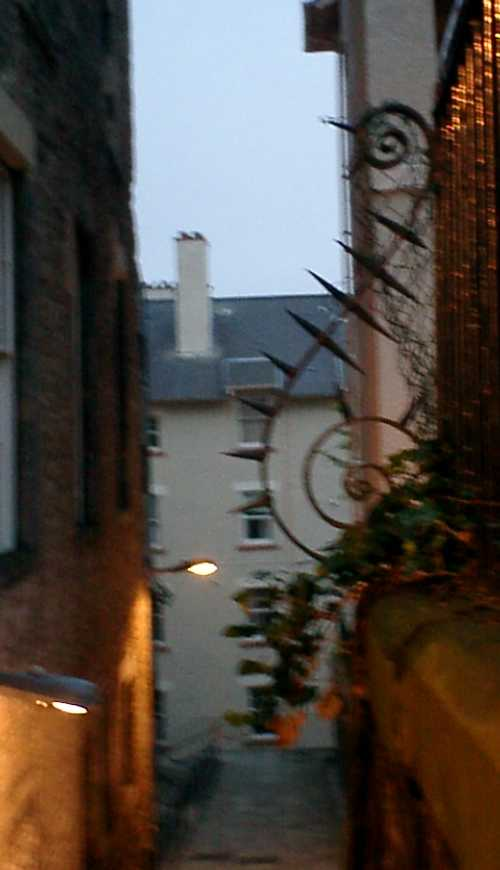
\includegraphics[width=1\hsize]{image200707/gurutitle.jpg}
\end{minipage}
\begin{minipage}{0.39\hsize}
 {\Huge #1
 }
\end{minipage}
\end{frame}
}

% 三択問題用
\newcounter{santakucounter}
\newcommand{\santaku}[5]{%
\addtocounter{santakucounter}{1}
\frame{\frametitle{問題\arabic{santakucounter}. #1}
%問題\arabic{santakucounter}. #1
\begin{minipage}[t]{0.8\hsize}
 \begin{itemize}
 \item
      \begin{minipage}{0.2\hsize}
      
\includegraphics[width=0.9\hsize]{image200703/janken-A.png}\end{minipage} 
       \begin{minipage}{0.6\hsize}
       A #2\end{minipage}\\
 \item
      \begin{minipage}{0.2\hsize}
      
\includegraphics[width=0.9\hsize]{image200703/janken-B.png}\end{minipage} 
       \begin{minipage}{0.6\hsize}
       B #3\end{minipage}\\
 \item
      \begin{minipage}{0.2\hsize}
      
\includegraphics[width=0.9\hsize]{image200703/janken-C.png}\end{minipage} 
       \begin{minipage}{0.6\hsize}
       C #4\end{minipage}\\
 \end{itemize}
\end{minipage}
}
\frame{\frametitle{問題\arabic{santakucounter}. #1}
%問題\arabic{santakucounter}. #1
\begin{minipage}[t]{0.8\hsize}
\begin{itemize}
 \item
      \begin{minipage}{0.2\hsize}
      
\includegraphics[width=0.9\hsize]{image200703/janken-A.png}\end{minipage} 
       \begin{minipage}{0.6\hsize}
       A #2\end{minipage}\\
 \item
      \begin{minipage}{0.2\hsize}
      
\includegraphics[width=0.9\hsize]{image200703/janken-B.png}\end{minipage} 
       \begin{minipage}{0.6\hsize}
       B #3\end{minipage}\\
 \item
      \begin{minipage}{0.2\hsize}
      
\includegraphics[width=0.9\hsize]{image200703/janken-C.png}\end{minipage} 
       \begin{minipage}{0.6\hsize}
       C #4\end{minipage}\\
\end{itemize}
\end{minipage}
\begin{minipage}[t]{0.15\hsize}
答えは:

\vspace{1cm}

  {\huge \hspace{1cm}#5}
  \hspace{-6cm}\includegraphics[width=4cm]{image200703/janken-#5.png}
 \end{minipage}}
}

\begin{document}
\frame{\titlepage{}}

\section{live-helper}

\begin{frame}
\frametitle{live-helper とは?}
\begin{itemize}
\item Debian pakcage を使った Live-CD 作成ツール
\item Google SoC の成果物の一つ
\item CD イメージだけではなく、 HDD イメージ、NFS イメージも作成できる
\end{itemize}
\end{frame}


\begin{frame}[containsverbatim]
\frametitle{インストール}
\begin{commandline}
% sudo apt-get install live-helper
\end{commandline}
or
\begin{commandline}
% sudo aptitude install live-helper
\end{commandline}

\begin{itemize}
\item etch ではサポートされておらず、 lenny , sid を使う必要がある。
\item etch で使う場合は backports.org を利用することにより、使用可能。
\end{itemize}
\end{frame}

\begin{frame}
\frametitle{使い方}
使い方は非常にシンプル。
\begin{itemize}%[<+->]
\item<1-> lh\_config

  live-helper の初期化および設定
\item<2-> lh\_build

  イメージ作成

\item<3-> lh\_clean

  キャッシュファイル等を削除
\end{itemize}
\end{frame}

\begin{frame}
\frametitle{lh\_config}
lh\_config を実行した後、config ディレクトリ以下に以下のファイルが作成される。
\begin{tabular}{|c|c|}
\hline
ディレクトリ名 & 説明 \\ \hline \hline
binary & 作成される Live-CD イメージに関する設定\\ \hline
bootstrap & Live-CD 作成環境に関する設定\\ \hline
chroot & Live-CD のユーザーランドに関する設定\\ \hline
common & live-helper の基本設定\\ \hline
source & source イメージに関する設定\\ \hline
\end{tabular}
\pause
\\
これらのファイルに各設定がかかれており、設定するために {\color{red} lh\_config}を使う。\\
現在の設定可能項目は 78項目。
\end{frame}

\begin{frame}[containsverbatim]
\frametitle{lh\_config 相談例 1}
\begin{center}\large
えっちな の Live-CD を作りたいんですが。
\end{center}
\end{frame}

\begin{frame}[containsverbatim]
\frametitle{lh\_config 相談例 1}
\large
\begin{itemize}
\item 実行
\begin{commandline}
% lh_config --distribution etch
% sudo lh_build
\end{commandline}

\item 設定ファイル
\begin{commandline}
config/bootstrap:LH_DISTRIBUTION="lenny"
\end{commandline}
が
\begin{commandline}
config/bootstrap:LH_DISTRIBUTION="etch"
\end{commandline}
に変更される。

\end{itemize}
\end{frame}

\begin{frame}[containsverbatim]
\frametitle{lh\_config 相談例 2}
\begin{center}\large
CD boot 時に萌え萌えな画像を出したいんですが。
\end{center}
\end{frame}

\begin{frame}[containsverbatim]
\frametitle{lh\_config 相談例 2}

\large
\begin{itemize}
\item 実行
\begin{commandline}
% lh_config --syslinux-splash= 
  "/home/uekawa/お気に入り/萌え萌えな画像014.jpg"
% sudo lh_build
\end{commandline}

\item ファイル
\begin{commandline}
config/binary:LH_SYSLINUX_SPLASH=""
\end{commandline}
が
\begin{commandline}
config/binary:LH_SYSLINUX_SPLASH=
"/home/uekawa/お気に入り/萌え萌えな画像014.jpg"
\end{commandline}
に変更される。
\end{itemize}
\end{frame}


%\begin{frame}
%\frametitle{オプションと設定項目}
%オプションと設定項目名は LH\_XXXXX として同じ名前になっています。
%\end{frame}

\begin{frame}[containsverbatim]
\frametitle{lh\_config を使用しない設定方法}
lh\_config は 環境変数も見ている。あらかじめ、環境変数に
値を設定して、動作させることも可能。
\begin{commandline}
% export LH_DISTRIBUTION=etch
% sudo lh_build
\end{commandline}

設定ファイルの内容が優先されるので注意。
\end{frame}

\begin{frame}
\frametitle{独自のパッケージをインストールしたい}
独自のパッケージをインストールするには、以下の手順を踏む必要がある。 \\

\begin{enumerate}
  \item 独自パッケージ用の apt-line を用意する
  \item config/chroot\_sources/moge.bootstrapに用意した apt-line を設定する
  \item config/chroot\_local-packageslists/ に適当なファイルを作成し、インストールしたいパッケージ名を列挙する。
\end{enumerate}
\pause 


このあたりは lh\_config ではできないっぽい。
\end{frame}

\begin{frame}[containsverbatim]
\frametitle{パッケージリストの活用}
ある程度の固まった環境を構築することができる、パッケージをまとめたもの。

\begin{commandline}
% ls /usr/share/live-helper/lists/
devel-live  gnome-core  gnome-junior  junior-pkgs  kde-core   
kde-full    knoppix     minimal       standard     studio 
studio-kde  xfce        gnome         gnome-full   gnustep       
kde         kde-extra   kde-junior    knoppix-dvd  rescue
standard-x11  studio-gnome  studio-xfce  xfce-junior
\end{commandline}


\begin{commandline}
% lh_config --packages-lists gnome-desktop
% sudo lh_build 
\end{commandline}
\end{frame}

\begin{frame}[containsverbatim]
\frametitle{パッケージ化されていないソフトウェアの追加方法}

\begin{enumerate}
\item chroot\_local-includes/content/ ディレクトリを作成
\item chroot\_local-includes/content/ にインストールしたいデータをコピー
\end{enumerate}


例: usr/bin/に hello\_world というプログラムを追加したい場合は
\begin{commandline}
chroot_local-includes/content/usr/bin/hello_world
\end{commandline}
にコピーする。
\end{frame}

\begin{frame}
コマンドラインなんて使えないんだよ!という人のために
\end{frame}

\begin{frame}
\frametitle{live-magic}
\begin{center}
  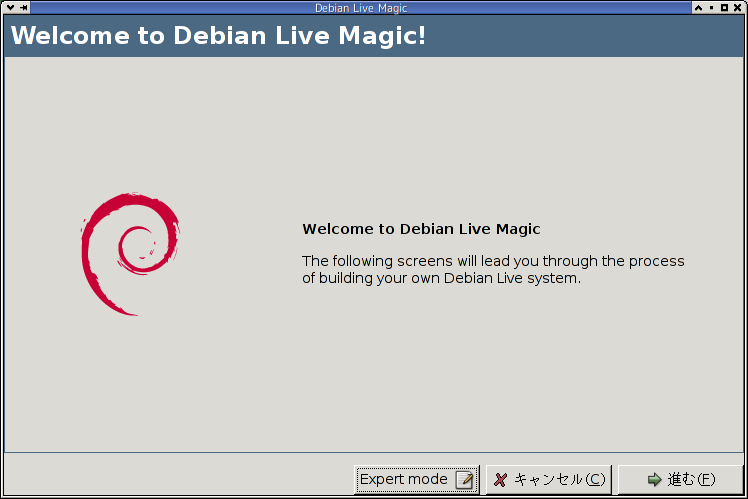
\includegraphics[width=0.8\hsize]{image200711/live-magic00.png}
\end{center}
\begin{itemize}
\item live-helper の GUI フロントエンド
\item python/gtk で書かれている。
\end{itemize}
\end{frame}

%\section{他の Live-CD との違い}
%\begin{frame}
%\frametitle{他の Live-CD}
%\begin{itemize}
%\item オリジナルのツールを使ってカスタマイズしている。
%
%  といっても、オリジナルをloopback 
%\item 基本的にすべて手作業。
%\item カスタマイズめんどい。
%\end{itemize}
%\end{frame}

\begin{frame}
\frametitle{今後の課題}
\begin{enumerate}
\item etch との相性が悪い
\item カーネルまわりで不具合が多いので修正したいところ
\item 日本語環境のサポート

  パッケージリストに 日本語環境入れたい。

\item HDD へのインストーラー
\end{enumerate}
\end{frame}


\begin{frame}
\frametitle{live-helper を使ったディストリビューション}
\begin{itemize}
\item Debian Live

  \url{http://debian-live.alioth.debian.org/}
\item Makai

  \url{http://makai.sourceforge.jp/wiki/}
\item dcastkit

  \url{https://ssl.keshi.org/projects/dcastkit/trac.fcgi}
\end{itemize}

\end{frame}


\begin{frame}
\frametitle{その他情報}
\begin{itemize}
\item live-helper webサイト

  \url{http://debian-live.alioth.debian.org/}
\item wiki

  \url{http://wiki.debian.org/DebianLive/}
\end{itemize}
\end{frame}



\end{document}
